\section{Numerical Ordinary Differential Equations}

\subsection{Definitions}
Ordinary Differential Equation (ODE):
$$\boxed{y'(x) = f(x,y(x)) \qquad\text{with}\qquad y(x_0) = y_0}$$
$f(x,y)$ is also referred to as the right-hand side (r.h.s.) function.

\subsection{Explicit Methods}
\label{sec:ode_explicit_methods}
Forward time stepping is used without the need for solvers, based on the Taylor approximation.
However, this approach becomes computationally intensive quickly,
requiring higher derivatives in multiple dimensions.

$$\boxed{y(x_0+h) = y(x_0) + \frac{h}{1!} y'(x_0) + \frac{h^2}{2!}y''(x_0) + \ldots + \frac{h^p}{p!}y^{(p)}(x_0) +\underset{\text{remainder term}}{\underbrace{ \frac{h^{p+1}}{(p+1)!}y^{(p+1)}(\xi)}}}$$

Further derivatives are derived using the chain rule:
$$\boxed{y''(x) = \frac{\partial f(x,y)}{\partial x} 1 + \frac{\partial f(x,y)}{\partial y}f(x,y) = \frac{\partial y'(x)}{\partial x} 1 + \frac{\partial y'(x)}{\partial y}y'(x)} \quad
\boxed{y'''(x) = \frac{\partial y''(x)}{\partial x} 1 + \frac{\partial y''(x)}{\partial y}y'(x)} \quad \ldots$$
Derivatives up to the third degree are listed here (immense computational effort required):

\begin{align*}
  y(x+h)=&	y(x)+\frac{f(x,y)}{1!}h+\\
    &\frac{1}{2!}\left(\frac{\partial f(x,y)}{\partial x} 1+ \frac{\partial f(x,y)}{\partial y} f(x,y)\right)h^2+\\
    &\frac{1}{3!}\left(\frac{\partial^2f(x,y)}{\partial x^2} 1+2\frac{\partial^2f(x,y)}{\partial x\partial y}f(x,y)+\frac{\partial^2f(x,y)}{\partial y^2} f(x,y)^2+\left(\frac{\partial f(x,y)}{\partial y}\right)^2 f(x,y)+\frac{\partial f(x,y)}{\partial x}\frac{\partial f(x,y)}{\partial y}\right)h^3+\ldots+\\
    &\frac{1}{4!}y^{(4)}(x)h^4+\ldots+\frac{1}{p!}y^{(p)}(x)h^p+\underbrace{\frac{1}{(p+1)!}y^{(p+1)}(\xi)h^{p+1}}_{\text{remainder term}}
\end{align*}

\begin{align*}
\text{Global error} &= \underbrace{\max}_{0 \leq i \leq k} |y_i - y(x_i)| \\
\text{Local error (slope)} &= \tau_h(x_n) = \frac{y(x_n +h)- y(x_n)}{h} - \left( \frac{y'(x_n)}{1!} + \frac{y''(x_n)}{2!}h^1 + \dots + \frac{y^{(p)} (x_n)}{p!} h^{p-1} \right) \\
h \tau_h(x_n) &= y(x_n +h)- y(x_n) - \left( \frac{y'(x_n)}{1!}h^1 + \frac{y''(x_n)}{2!}h^2 + \dots + \frac{y^{(p)} (x_n)}{p!} h^{p} \right)
\end{align*}

Assuming that the initial value of the current step is exactly correct, i.e., $y_n = y(x_n)$:
$$h \tau_h(x_n) = y(x_n +h) - \left(y(x_n) + \frac{y'(x_n)}{1!}h^1 + \frac{y''(x_n)}{2!}h^2 + \dots + \frac{y^{(p)} (x_n)}{p!} h^{p} \right) = y(x_n + h)-y_{n+1}$$

\begin{minipage}{7cm}
  \subsubsection{Explicit Euler Method}
    Special case of explicit methods: \\
    \emph{Taylor with order $p=1$} \\
    Relatively inaccurate approximation since the derivative remains unchanged in each step.  \\

    Global error: $\max_{0 \leq i \leq k} |y_i - y(x_i)|$ with the number of steps $k$\\
    Local error: $y(x_n+h) - y_{n+1}$ when the initial value of the current step is exactly correct
\end{minipage}
\hspace{8mm}
\begin{minipage}{12cm}
    \begin{align*}
        y_0 &= y(x_0) \\
        y(x_0+h) \approx y_1 &= y_0 + f(x_0,y_0) h \approx y(x_0) + y'(x_0)h \\
        y(x_1+h) \approx y_2 &= y_1 + f(x_1,y_1)h \approx y(x_1) + y'(x_1)h \\
        & \vdots \\
        y(x_{n-1}+h) \approx y_n &= y_{n-1} + f(x_{n-1},y_{n-1})h \approx y(x_{n-1}) + y'(x_{n-1})h
    \end{align*}
\end{minipage}

\subsubsection{Explicit Taylor Methods of Higher Order}
  For $p > 1$, a better approximation is achieved, but the computational effort increases significantly.
  See Section \ref{sec:ode_explicit_methods} for calculation.

  \begin{align*}
      y_0 &= y(x_0) \\
      y_{k+1} &= y_k + \frac{y_k'}{1!}h_k + \frac{y_k''}{2!} h_k^2 + \ldots + \frac{y_k^{(p)}}{p!} h_k^p
  \end{align*}

\newpage
    \skriptsubsubsection{Explicit Runge-Kutta (RK) Methods}{8}
    $s$ recursive stages $k$ are defined, which, when summed, yield the Taylor approximation. Here, $s=4$.
    \begin{align*}
        k_1 &= hf(x,y)\\
        k_2 &= hf(x + m h, y+m k_1)\\
        k_3 &= hf(x + n h, y+n  k_2)\\
        k_4 &= hf(x + p h, y+p k_3)
    \end{align*}
    $$y(x+h) \approx y(x) + a k_1 + b k_2 + c k_3 + d k_4 $$
    In contrast to the script (p. 10), the $h$ values are not included in the $k$ definitions but appear in the final formula. With the correct boundary conditions (p. 11), this formula corresponds to the Taylor polynomial up to order 4.

    By equating with Taylor, explicit RK methods define an overdetermined system of equations with 8 equations and 7 unknowns $m,n,p$ and $a,b,c,d$.

    There are different \textbf{solutions}, also listed here for order $s=2$ and $s=4$:
    \begin{tabular}{lll}
        Solution Name & \# Stages ($s$) & Solutions\\
        Heun & 2 & $a=b=\frac12$, $m=1$ ($n=p=c=d=0$)\\
        Explicit Midpoint & 2 & $a=0$, $b=1$, $m=\frac12$ ($n=p=c=d=0$)\\
        Classical Runge-Kutta & 4 & $m=n=\frac12$, $p=1$, $a=d=\frac16$, $b=c=\frac13$
    \end{tabular}

    $$
    \text{Local error (slope)} = \tau_h(x_n) = \frac{y(x_n +h)- y(x_n)}{h} - \left( \frac{\tilde k_1 + 2\tilde k_2 +2 \tilde k_3 + \tilde k_4}{6h} \right)
    $$
    The tilde superscript $\tilde k$ indicates that the stage values $k$ must be evaluated using exact values for $x$, $y$.

\skriptsubsubsection{General Framework for Runge-Kutta Methods (Butcher Tableaus)}{13}
    \begin{minipage}{6cm}
        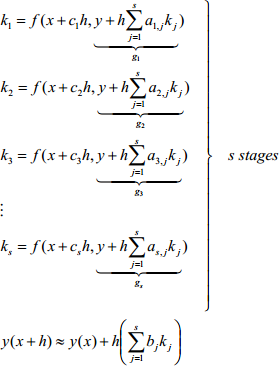
\includegraphics[width=5cm]{./bilder/ode_rungekutta_framework1.png}
    \end{minipage}
    \begin{minipage}{4.5cm}
        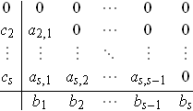
\includegraphics[width=3cm]{./bilder/ode_rungekutta_butcher.png}\\
        $\bm a$ = Splitting in $Y$\\
        $\bm b^T$ = Solutions given by the method\\
        $\bm c$ = Splitting in $X$\\

        FSAL (First Same As Last) Special Form:\\
        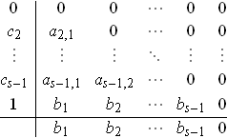
\includegraphics[width=3cm]{./bilder/butcher_fsal.png}
    \end{minipage}
    \hspace{0.5cm}
    \begin{minipage}{9cm}
        Conditions (For Explicit Method):
        \begin{itemize}
            \item $c_i = \sum\limits_{j=1}^s a_{ij} = \sum\limits_{j=1}^{i-1} a_{ij}\,(i=2,\ldots,s)$
            \item $\sum\limits_{j=1}^s b_j = 1$
            \item $c_1=0$
            \item $a_{1j} = 0 \quad 1\leq j\leq s $
            \item $a_{ij} = 0 \quad j\geq i$
        \end{itemize}
        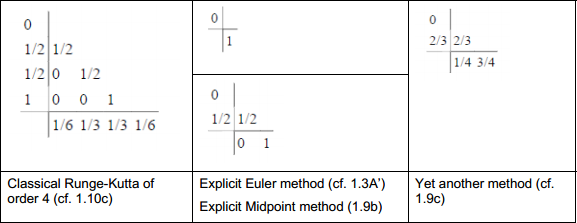
\includegraphics[width=8cm]{./bilder/ode_rungekutta_butcher_examples.png}\\
        Heun Method (RK-2): $b_1 = b_2 = \frac{1}{2}; c_2=\frac{1}{2}; a_{2,1}=\frac{1}{2}$
    \end{minipage}

    \begin{center}
        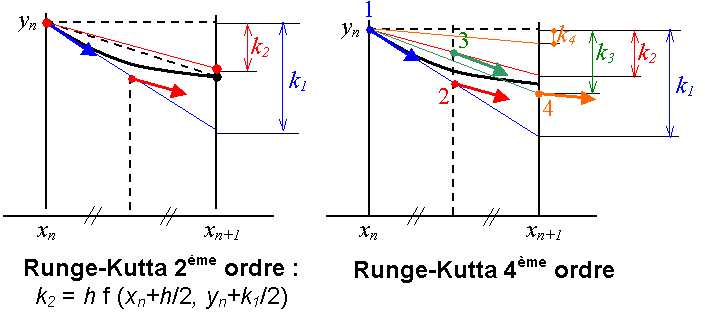
\includegraphics[width=0.6\linewidth]{bilder/rungekutta.png}
    \end{center}

\newpage
\skriptsubsubsection{Adaptive Explicit Methods}{17}
    Idea: Automatic adaptation of the step size $h$. This requires defining the maximum error of the approximation. The \emph{Accuracy Goal} ($ag$) specifies the minimum matching number of decimal places, while the \emph{Precision Goal} ($pg$) represents the number of significant figures in the result. The tolerance parameter is:
    $$\varepsilon = \varepsilon_a+ |y|\varepsilon_r=10^{-ag} + |y| 10^{-pg} \geq |e|.$$

    \subsubsubsection{Embedded Pairs of Explicit Runge-Kutta Methods}\\
    \begin{minipage}{5cm}
        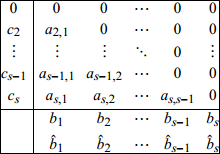
\includegraphics[width=4cm]{./bilder/ode_adaptive_butcher.png}
    \end{minipage}
    \begin{minipage}{13cm}
        The method introduces a second approximation, an \emph{embedded order} $\hat{p}$, responsible for error calculation. The \emph{primary order} $p$ is required to calculate the step size. Usually, $\hat{p} = p-1$.

        The Butcher tableau is expanded by a row of $b$ numbers.
    \end{minipage}\\

    Local error:
    $$e_n = y(x+h) - \hat{y}(x+h) = h_n \sum\limits_{j=1}^s (b_j - \hat{b}_j)k_j \Rightarrow
    \Arrowvert e_n \Arrowvert = \left\Arrowvert h_n \sum\limits_{j=1}^s (b_j - \hat{b}_j)k_j \right\Arrowvert$$

    \begin{minipage}{7.5cm}
        If at the current step $\boxed{\frac{\Arrowvert e_n \Arrowvert}{\varepsilon} > 1}$, then the estimation of $h_n$ was too optimistic, and the step must be repeated with a smaller step size (\textbf{Reject}).

        Otherwise $\boxed{\frac{\Arrowvert e_n \Arrowvert}{\varepsilon} \leq 1}$, continue with the step size update (\textbf{Proceed}):

        $$h_{n+1} = h_n \left( \frac{\varepsilon}{\Arrowvert e_n \Arrowvert} \right)^{\frac{1}{\tilde{p}}}=
        h_n \left( \frac{\Arrowvert e_n \Arrowvert}{\varepsilon} \right)^{-\frac{1}{\tilde{p}}}$$
        $$\varepsilon=\varepsilon_a+\varepsilon_r|y_n|
        \text{\qquad with\quad} \tilde{p} = \min(p, \hat{p})+1 \text{ (Order of the primary method)}$$
    \end{minipage}
    \hspace{0.5cm}
    \begin{minipage}{10.5cm}
        \subsubsubsection{Example}\\
        \begin{tabular}{cccccc}
            \hline
            $x$ & $\bm y$ & $h_n$ & $\left( \frac{\Arrowvert e_n \Arrowvert}{\varepsilon} \right)^{-\frac{1}{\tilde{p}}}$ & $h_{n+1}$ & Status \\
            \hline
            $10$ & $[1, -1]^T$ & 1 & 0.4 & 0.4 & Reject\\
            10 & $[1,-1]^T$ & 0.4 & 1.5 & 0.6 & Proceed\\
            10.4 & $[0.420958, -1.40852]^T$ & 0.6 & 0.5 & 0.3 & Reject\\
            \hline
        \end{tabular}
    \end{minipage}

\skriptsubsubsection{Stability of Explicit Methods}{27}
  The global relative error must not diverge; it must be bounded. Since the analysis with the ODE under investigation is challenging due to the lack of knowledge about the solution, the general ODE is considered, the Dahlquist model:
  $$y' = A y \quad y(0) = 1 \qquad \text{with } A = \Re\{A\} + j \Im\{A\} \in \mathbb{C}$$
  Its solution is $y = e^{\Re\{A\} x} \left( \cos(\Im\{A\}x) + j \sin(\Im\{A\} x) \right)$, i.e., a vibration with exponential amplitude $e^{\Re\{A\} x}$ and frequency $\Im\{A\}$.

  With the method under investigation, a \emph{linear stability function} $F(z)$ can be calculated.

  \subsubsubsection{Example} The examination is shown using the Heun method (RK-2):
  \begin{align*}
      k_1 &= A y_k                                          & y_0 &= y(x_0) = y(0) = 1\\
      k_2 &= A(y_k + 1 h k_1) = A(y_k + Ah y_k) \qquad \Longrightarrow &
      y_{k+1} &= y_k \underbrace{\left(1 + hA + (hA)^2 \frac12\right)}_{F(hA) = F(z), \quad z=hA \in \mathbb{C}}
  \end{align*}
  The linear stability function can now be substituted as follows:
  $$y_{k+1} = \Big( | F(z) | \exp \big(j \arg(F(z))\big) \Big) y_k$$

  \begin{minipage}{10cm}
      Now three cases can be distinguished:
      \begin{enumerate}
          \item $\Re\{A\} < 0$: The amplitude of the ODE decreases exponentially. The stability condition requires that the approximated values $y_k$ ($k=0,1,\ldots$) also decrease exponentially. Therefore, and from $y_{k+1} \propto | F(z) |$, it follows that $|F(z)| < 1$.
          \item $\Re\{A\} = 0$: The amplitude of the ODE is constantly 1. The stability condition requires that the approximated values $y_k$ ($k=0,1,\ldots$) also remain constant. Therefore, and from $y_{k+1} \propto | F(z) |$, it follows that $|F(z)| = 1$.
          \item $\Re\{A\} > 0$: The amplitude of the ODE increases exponentially. The stability condition requires that the approximated values $y_k$ ($k=0,1,\ldots$) also increase exponentially. Therefore, and from $y_{k+1} \propto | F(z) |$, it follows that $|F(z)| > 1$.
      \end{enumerate}

      Cases 2 and 3 do not pose problems (conditions are always fulfilled); only the first case is critical.
  \end{minipage}
  \hspace{1cm}
  \begin{minipage}{8cm}
      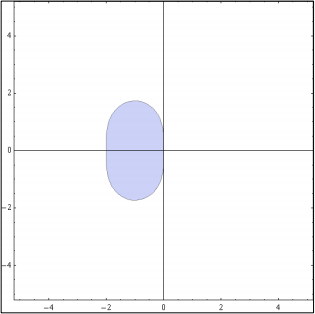
\includegraphics[width=6cm]{./bilder/ode_stability_heun.png}\\
      Case 1 of the stability condition ($\Re\{A\} < 0$): \\
      $1 > |F(z)| = |1 + hA + \frac12 (hA)^2| \Rightarrow -2 < h \Re\{A\} < 0$.\\
      Cases 2 and 3 are not considered in the figure.
  \end{minipage}

  \vspace{1em}
  \subsubsubsection{Recursive Formula} \formelbuch{29}
      Recursive formulas exist for the stability polynomial $F(z) = 1 + b_1 k_1(z) + \ldots + b_sk_s(z)$:\\
      $k_1(z) = z, \qquad k_{j+1}(z) = z(1 + a_{j+1,1} k_1(z) + a_{j+1,2} k_2(z) + \ldots + a_{j+1,j} k_j(z))$

  \vspace{1em}
  \subsubsubsection{Weakness of Explicit Methods}: Stability!

\skriptsubsubsection{Stiffness}{33}
  Definition: Stiffness = very challenging (according to Wikipedia). Rough idea: Explicit methods are forced to unacceptably small step sizes (computational complexity). This happens despite the actual "smooth" surfaces of the functions, which should intuitively not be very difficult to calculate.\\

  If stability violations (stiffness) are detected, a switch to implicit methods (black-box solvers) should be made, and then, with non-stiffness detection, a switch back to explicit methods should be made.\\

  Stiffness depends on:
  \begin{enumerate}
      \item Specific ODE
      \item Specific step size $h$
      \item Specific method (e.g., RK-4)
  \end{enumerate}

  \subsubsubsection{Stiffness Detection}
  Requirement: $c_{s-1} = c_s = 1$. Stiffness can be detected by testing $\left|h \frac{\partial f(x,y)}{\partial y} \right|$ against the absolute limit of the stability region. Stiffness is present if $|h \tilde{\lambda}|$ is outside or on the boundary of the stability region.

  Example of explicit Runge-Kutta:
  $$k_{s-1} = f(x+c_{s-1} h, \underbrace{y + h \sum\limits_{j=1}^s a_{s-1,j}k_j}_{g_{s-1}}) \qquad
  k_{s} = f(x+c_{s} h, \underbrace{y + h \sum\limits_{j=1}^s a_{s,j}k_j}_{g_{s}}) \qquad
  \Rightarrow \qquad \tilde{\lambda} = \frac{\Arrowvert k_s - k_{s-1} \Arrowvert}{\Arrowvert g_s - g_{s-1} \Arrowvert}$$

  $\tilde{\lambda}$ is an estimate for $f_y = \frac{\partial}{\partial y}f(x,y)$, e.g., $y'=x^4-25y^4=f(x,y)$, and takes on the role of $\Re \{A\}$ in stability analysis.

\skriptsubsection{Systems of ODEs and Higher-Order ODEs}{37}
  Systems of ODEs are written in vector notation and calculated as usual. That's all.
